\section{PackStack Install}
\label{app:packstack-install}

This section covers the commands used to install OpenStack PackStack and 
any configuration changes to the host machine needed to accommodate the
install. For configuration of the OpenStack deployment please see
Appendix~\ref{app:packstack-config}.

\subsection{Network Configuration}
\label{host-network-config}
Before running any installation commands it is necessary to understand
the initial network configuration and target network configuration. The
initial network configuration can be seen below in
Figure~\ref{fig:initial-network}. The host machine has two IP addresses,
one for accessing storage on VLAN 23 with address 10.23.10.10 and one
for accessing the Internet on VLAN 26 with address 10.26.10.10. Each of
these VLAN interfaces are attached to the single device interface for
enp4s0f1.

\begin{figure}[H]
  \centering
  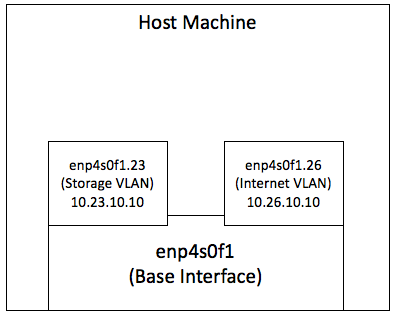
\includegraphics[scale=0.5]{img/initial-network}
  \caption{Initial network device diagram on the host machine.}
  \label{fig:initial-network}
\end{figure}

The following contains the content of the initial configuration for each
of the three devices pictured in Figure~\ref{fig:initial-network},
enp4sf01, enp4sf01.23, and enp4sf01.26.\\
\textbf{Initial contents of /etc/sysconfig/network-scripts/ifcfg-enp4s0f1}
\verbatiminput{network-configs/base-old}
\textbf{Initial contents of /etc/sysconfig/network-scripts/ifcfg-enp4s0f1.23}
\verbatiminput{network-configs/vlan23-old}
\textbf{Initial contents of /etc/sysconfig/network-scripts/ifcfg-enp4s0f1.23}
\verbatiminput{network-configs/vlan26-old}

When PackStack is installed, it will create its own isolated networking
environment. If guest virtual machines want access to the Internet the
must be given an IP address on the 10.26.10.0/24 network. However,
giving an IP address to these machines is not enough, the interfaces
created by PackStack must be configured to route traffic through the
existing networking infrastructure to the Internet.
Figure~\ref{fig:modified-network} shows a high level overview of the
networking devices configured by PackStack and the modifications made to
the host machine to accommodate routing guest traffic to the Internet.

\begin{figure}[H]
  \centering
  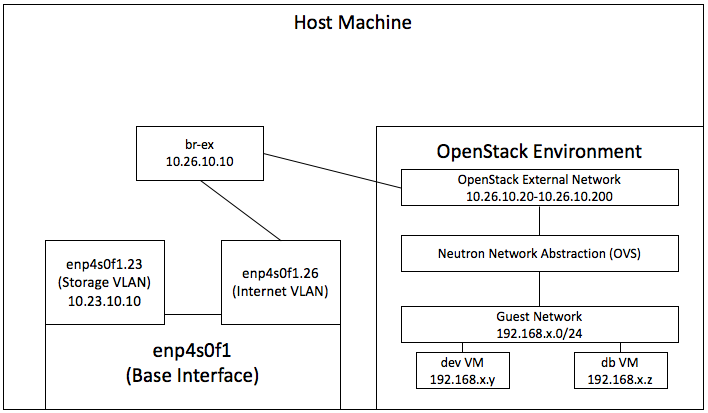
\includegraphics[scale=0.5]{img/modified-network}
  \caption{Modified network device diagram on the host machine and internal to PackStack.}
  \label{fig:modified-network}
\end{figure}

Here we see the guest network is an isolated 192.168.0.0/16 network. If
a VM on this network wishes to reach the Internet, it must be given an
IP address from the OpenStack External Network, which is handled by
Neutron. From here traffic must be forwarded to the host machine and
sent out on the 10.26.10.10 address to the Internet, however to
accommodate this it was necessary to create a bridge interface named
br-ex and assign it the IP address. This bridge interface connects the
host network with the OpenStack External Network. With this
configuration, guest may ask for External IPs and then connect to the
Internet from the guest or SSH into the guest from inside the Oscar Lab
network.

This can be rather unintuitive since all IP addresses are actually private
reserved IP addresses, but all NAT and packet forwarding is done
transparently to the user to make it seem as if the guest VM has been
assigned a public IP address. First the Oscar Lab router routes the packet
to the host machine, then NAT is applied at the host to route the packet to
the guest VM inside OpenStack. The only caveat to the approach of using
private reserved IP address as external public addresses, is the guest VM
cannot be directly routed to from the outside world, which works as a
security feature as discussed in the design section on security (Section
~\ref{sec:security}).

The following contains the content of the modified and additional
network interface configurations, excluding those automatically
generated and maintained by PackStack.\\
\textbf{Modified contents of /etc/sysconfig/network-scripts/ifcfg-enp4s0f1.26}
\verbatiminput{network-configs/vlan26-new}
\textbf{Created contents of /etc/sysconfig/network-scripts/ifcfg-br-ex}
\verbatiminput{network-configs/br-ex}


\subsection{PackStack Installation}
\label{host-packstack-install}

With the networking properly planned and configured, installation of
PackStack can be done. Installation followed the RDO PackStack
Installation Guide~\cite{PackStacksetup}, with minor modifications for
the version of OpenStack in use.

First begin by adding the rdo repo, doing a system update, and
installing OpenStack PackStack
\begin{lstlisting}
  sudo yum install -y https://www.rdoproject.org/repos/rdo-release.rpm
  sudo yum update
  sudo yum upgrade
  sudo yum install openstack-packstack
\end{lstlisting}

Then run the PackStack install with the following configurations to
attach the OpenStack network to the existing network.
\begin{lstlisting}[escapechar=&]
  packstack &\texttt{--}&allinone &\texttt{--}&provision-demo=n \
  &\texttt{--}&os-neutron-ovs-bridge-mappings=extnet:br-ex \
  &\texttt{--}&os-neutron-ovs-bridge-interfaces=br-ex:enp4s0f1.26 \
  &\texttt{--}&os-neutron-ml2-type-drivers=vxlan,flat,vlan
\end{lstlisting}

After this command runs (this may take awhile), OpenStack is installed
and is ready to be customized.
